\chapter{Autonomous landing experiments}
The autonomous landing system has successfully been tested in the field, where the result from two subsequent days is presented. The landing plan that was test was only with a virtual net that was placed $26$ meters above the ground, using guidance and high level control systems in DUNE. The navigation system used \gls{rtk-gps} with the compensator system enabled, which ensures that the positioning of the \gls{uav} can be assumed highly accurate. The result of the navigation system is presented in section \ref{ss:EXNavigation}.
\section{Landing system}
The wind condition the first day had an windspeed at $8-9 m/s$ from west, and the second day was calm wind conditions at $1 m/s$ from west. Hence the performance of system was tested with two different wind condition, where one strained the performance of the system while the other could be considered as ideal conditions. The criteria used to indicate if the X8 would have hit the net is given in table \ref{tb:NetCriteria}, which is related to a net with the dimensions 3 meter height and 5 meter width. The virtual net was placed above a runway at Agdenes, such that the landing path is similar to a landing path where a physical net is used. All landing plan was generated when the \gls{uav} was in a loiter manoeuvre, such that the plan could be reviewed and the correct controllers assigned to the plan.
\begin{table}[H]
\centering
\begin{tabular}{| l | l |}
\hline
\textbf{Height acceptance}	& \textbf{Cross track error acceptance}	\\ \hline
$\pm1.5$					& $\pm2.5$								\\ \hline
\end{tabular}
\caption{Net hit acceptance criteria}
\label{tb:NetCriteria}
\end{table} 
\newpage
\subsection{Day 1}
The first plan created is shown in figure \ref{Fig:NorthEast31mai103029} and \ref{Fig:Height31mai103029}. The path created is design such that the \gls{uav} is brought into the crosswind, which strain the lateral controller and introduces oscillatory motion in the \gls{uav}.
 The \gls{uav} was set to loiter at a fixed point, from which the landing plan was generated. The lateral path of the \gls{uav} is shown in figure \ref{Fig:NorthEast31mai103029} and longitudinal path in \ref{Fig:Height31mai103029} with desired path and height respectfully.

The behaviour of the lateral path shown in figure \ref{Fig:NorthEast31mai103029} indicates that the lateral guidance system is struggling to hold the line when flying in the crosswind. When exiting the overshoot may cause the \gls{uav} to leave the line of sight of the pilot, in which case the only method of monitoring the \gls{uav} is over a radio link which can experience drop out. The behaviour of the \gls{uav} when flying keeps osculating around the straight line path, which is undesired during the finale stage of the landing plan. This behaviour can be reduced by lowering the lookahead distance in the lateral guidance system, however this will be at the cost of performance when flying parallel to the wind.

The longitudinal guidance system used outputs a desired heigh which lags behind the desired path due to a smoothing filter which is used to remove the discontinue between two line segments. The filter currently used will only converge to a constant height value, such that the net impact angle has to zero in order for the longitudinal guidance system to converge to the desired path height. A new landing plan, shown in figure \ref{Fig:Height31mai31mai105034} and \ref{Fig:NorthEast31mai105034}, was generated with the net impact angle $\gamma_n = 0$ which gave a better performance from the height guidance system. However this results in that the glide slope is the only part of the landing path where the height can be reduced, which will cause a problem when attempting to land in a real net. This is due to the length restriction of both the airfield and the operational area where the \gls{uav} is visible for the pilot. With the current landing plan and a landing direction from east the minimum height at which the \gls{uav} can starts its landing path is set to $56 m$ above ground. 
\newpage
\begin{figure}[H]
	\centering
		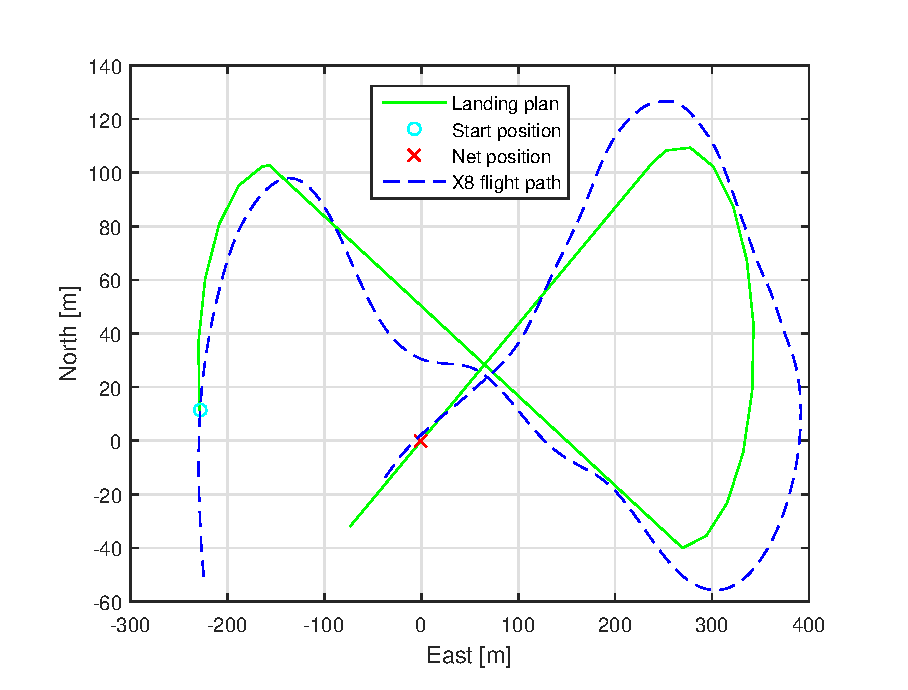
\includegraphics[scale=0.7]{figs/Experiment/NorthEast31mai103029.eps}
		\caption{North-East plot of a landing plan}
		\label{Fig:NorthEast31mai103029}
\end{figure}
\begin{figure}[H]
\centering
		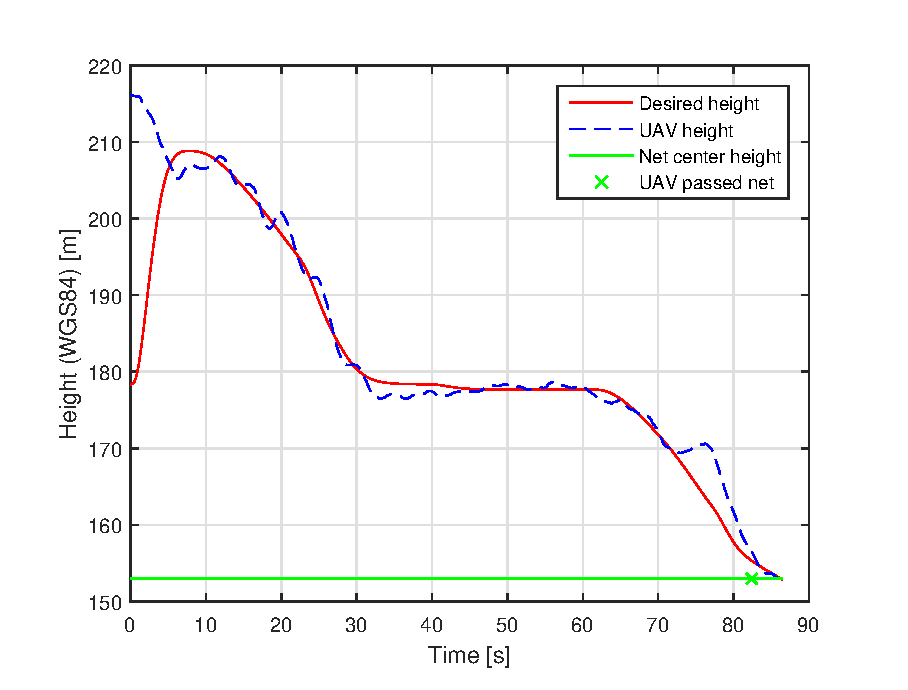
\includegraphics[scale=0.7]{figs/Experiment/Height31mai103029.eps}
		\caption{Height profile of landing plan with $3 \deg$ net impact angle}
		\label{Fig:Height31mai103029}
\end{figure}
During the new path the \gls{uav} was able to stay on the straight line towards the net. However the \gls{uav} still have oscillatory behaviour along the straight line connecting the two circles, with a large overshoot in the final turn. A better path would be to avoid flying in the cross wind as much as possible, which would result in a smoother path between the circles. However this will not remove the overshot in the final turn, all thought it will be reduced since the \gls{uav} is not in a oscillatory motion when entering the final circle. 

\begin{figure}[H]
	\centering
		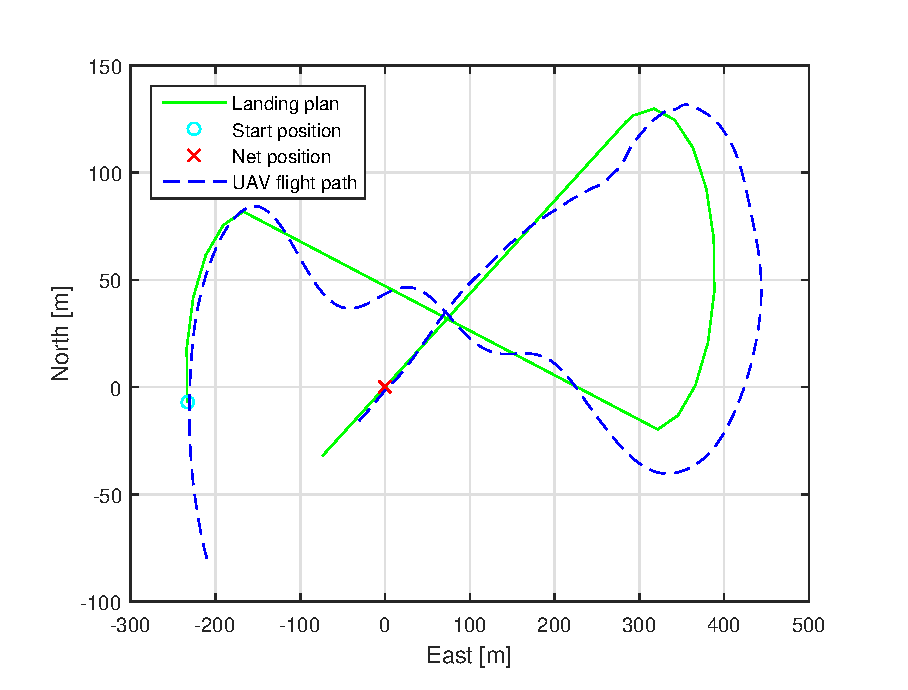
\includegraphics[scale=0.7]{figs/Experiment/NorthEast31mai105034.eps}
		\caption{North-East plot of a landing plan}
		\label{Fig:NorthEast31mai105034}
\end{figure}
\begin{figure}[H]
\centering
		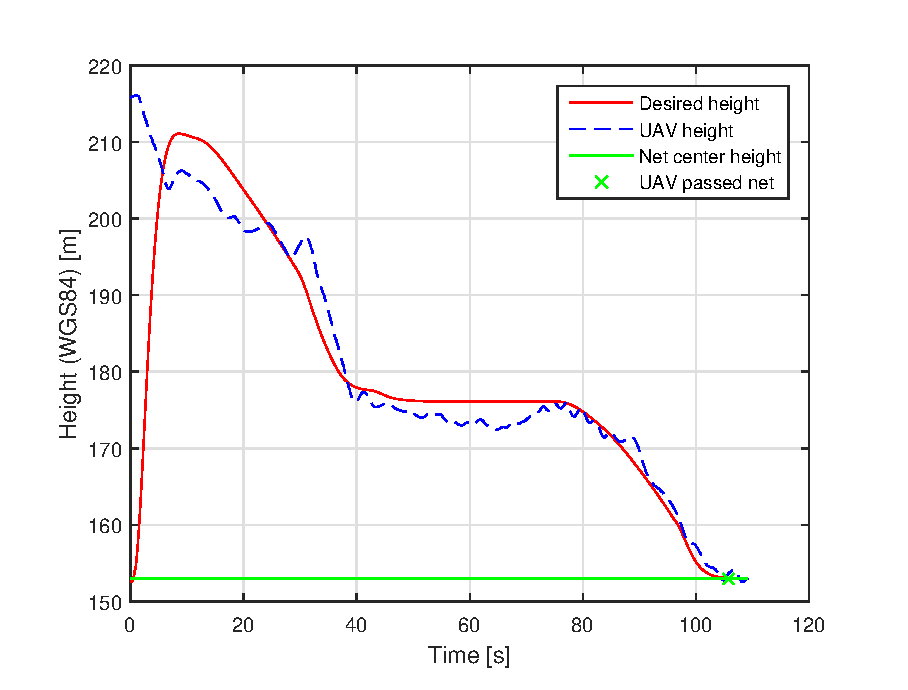
\includegraphics[scale=0.7]{figs/Experiment/Height31mai105034.eps}
		\caption{Height profile of landing plan with $0 \deg$ net impact angle}
		\label{Fig:Height31mai31mai105034}
\end{figure}
A new path was created where the rotation direction of the first circle was changed to counter clockwise, as shown in figure \ref{Fig:NorthEast31mai125420}. The new path had its straight line path between the circles parallel to the wind direction, which resulted in less oscillatory motion. However the overshoot in the final circle is still present, and is a result of the \gls{uav} attempting to turn up against the wind. Still the \gls{uav} struggle to keep to the straight line during along the landing path. In order to attempt to remove the oscillatory behaviour during the landing path the lookahead distance of the lateral controller was reduced such that the behaviour of the lateral controller becomes more aggressive. 
\begin{figure}[H]
	\centering
	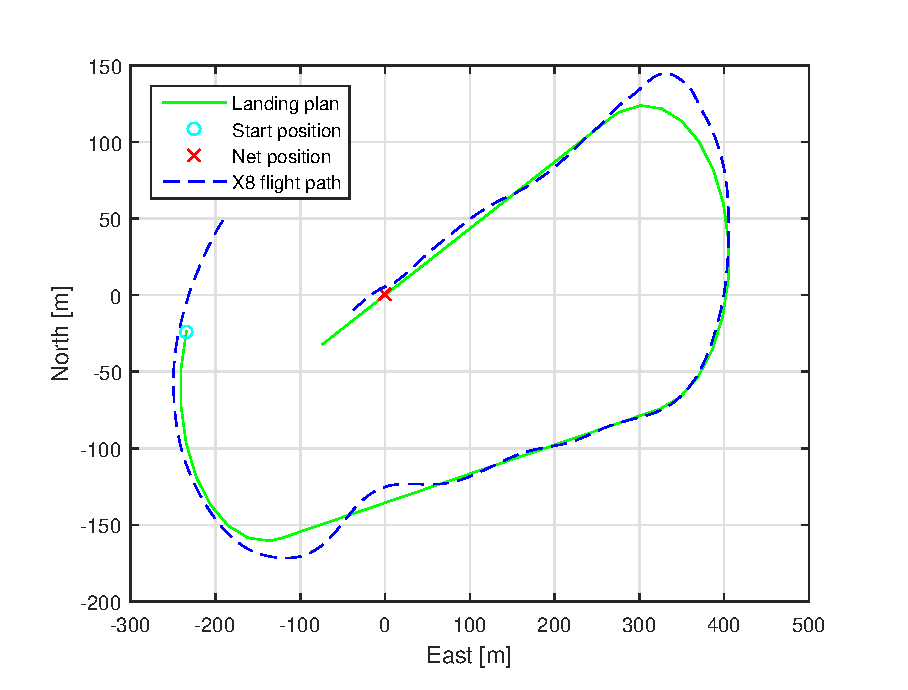
\includegraphics[scale=0.7]{figs/Experiment/NorthEast31mai125420.eps}
	\caption{North-East plot where the straight line segment between the two circles give a path parallel to the wind}
	\label{Fig:NorthEast31mai125420}
\end{figure}
A path where the lookahead distance of the lateral controller is reduced is shown in figure \ref{Fig:NorthEast31mai131844}. The \gls{uav} stays on the straight line towards the net, and the on the line between the circles it still has oscillatory motions, however this are reduced. 
\begin{figure}[H]
\centering
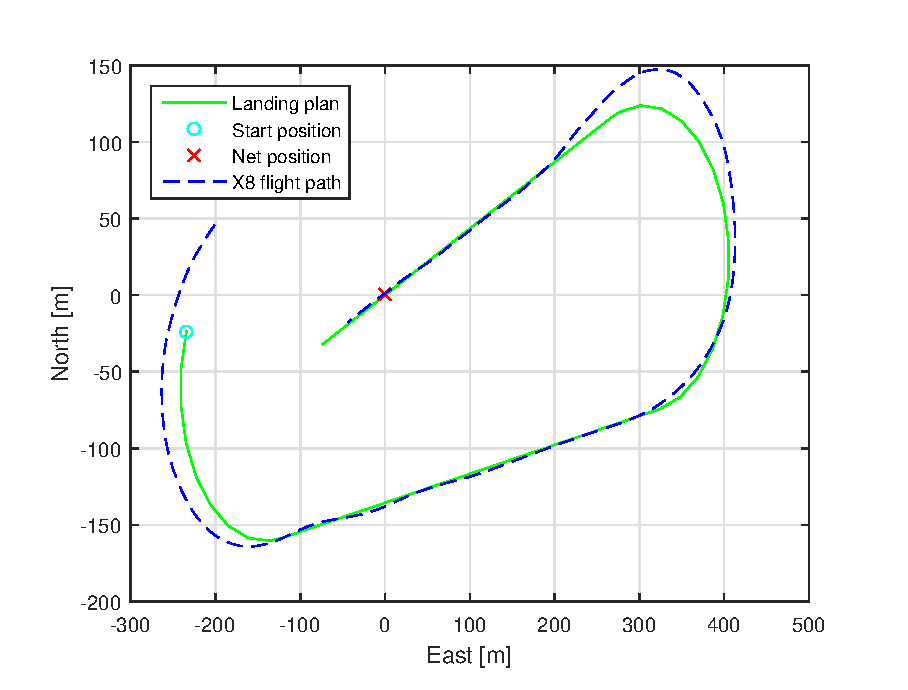
\includegraphics[scale=0.7]{figs/Experiment/NorthEast31mai131844.eps}
\caption{North-East plot where the lookahead distance of the lateral controller was reduced to increase performance when flying against the wind}
\label{Fig:NorthEast31mai131844}
\end{figure}
\subsubsection{Summary of day 1}
The result from the first day was affected with strong wind condition, in which the \gls{uav} struggled to stay on the path. The mean height and cross track error is listed in table \ref{tb:Day1HeightCrossTrack}, where the first column indicate the number of the landing attempt. As seen in table \ref{tb:Day1HeightCrossTrack} the average cross track error equals to $5.4 m$ 
\begin{table}[H]
\centering
\begin{tabular}{| l | l | l |}
\hline
\textbf{Nr.} 	& \textbf{Mean height error} 	& \textbf{Mean cross track error}  \\ \hline
$1$				& $1.5 m$							& $6.1 m$								\\ \hline
$2$				& $2.6 m$							& $6.7 m$								\\ \hline
$3$				& $0.9 m$							& $5.5 m$								\\ \hline
$4$				& $0.1 m$							& $2.8 m$								\\ \hline
$5$				& $1.7 m$							& $2.0 m$								\\ \hline
$6$				& $1.3 m$							& $6.8 m$								\\ \hline
$7$				& $1,8 m$							& $9.1 m$								\\ \hline
$8$				& $1.2 m$							& $8.2 m$								\\ \hline
$9$				& $1.9 m$							& $5.9 m$								\\ \hline
$10$			& $1.5 m$							& $4.4 m$								\\ \hline
$11$			& $1.5 m$							& $1.4 m$								\\ \hline
SUM				& $1.5 m$							& $5.4 m$								\\ \hline
\end{tabular}
\caption{Mean height and cross track error from day 1}
\label{tb:Day1HeightCrossTrack}
\end{table}
A table containing if a landing plan would result in a net landing is presented in table \ref{tb:Day1LandingAttempt}. The success rate of the first day gives a $36.3  \% $ probability of successfully landing in the net, which indicate that alteration to the current landing system is needed in order to achieve better performance in strong wind conditions.
\begin{table}[H]
\centering
\begin{tabular}{| p{0.5cm} | p{1cm} | p{1cm} | p{3.5cm} | p{3cm} | p{1cm} |}
\hline
\textbf{Nr.}	& \textbf{Height error [m]}	& \textbf{Cross track error [m]}& \textbf{Height acceptance}& \textbf{Cross track error acceptance}	& \textbf{Net hit}\\ \hline
$1$				& $2.8$		& $2.1$		& X								& OK									& X					\\ \hline
$2$				& $2.7$		& $-4.5$	& X								& X										& X					\\ \hline
$3$				& $0.9$		& $-1.6$	& OK							& OK									& OK				\\ \hline
$4$				& $0.0$		& $5.4$		& OK							& X										& X					\\ \hline
$5$				& $0.8$		& $5.$		& OK							& X										& X					\\ \hline
$6$				& $2.1$		& $-1.6$	& X								& OK									& X					\\ \hline
$7$				& $0.7$		& $2.3$		& OK							& OK									& OK				\\ \hline
$8$				& $-1.5$	& $-5.4$	& X								& X										& X					\\ \hline
$9$				& $1.9$		& $0.8$		& X								& OK									& X					\\ \hline
$10$			& $0.3m$	& $1.1$		& OK							& OK									& OK				\\ \hline
$11$			& $-1.3$	& $0.2$		& OK							& OK									& OK				\\ \hline
\end{tabular}
\caption{Table containing the result of each landing attempt}
\label{tb:Day1LandingAttempt}
\end{table}
\begin{figure}[H]
\centering
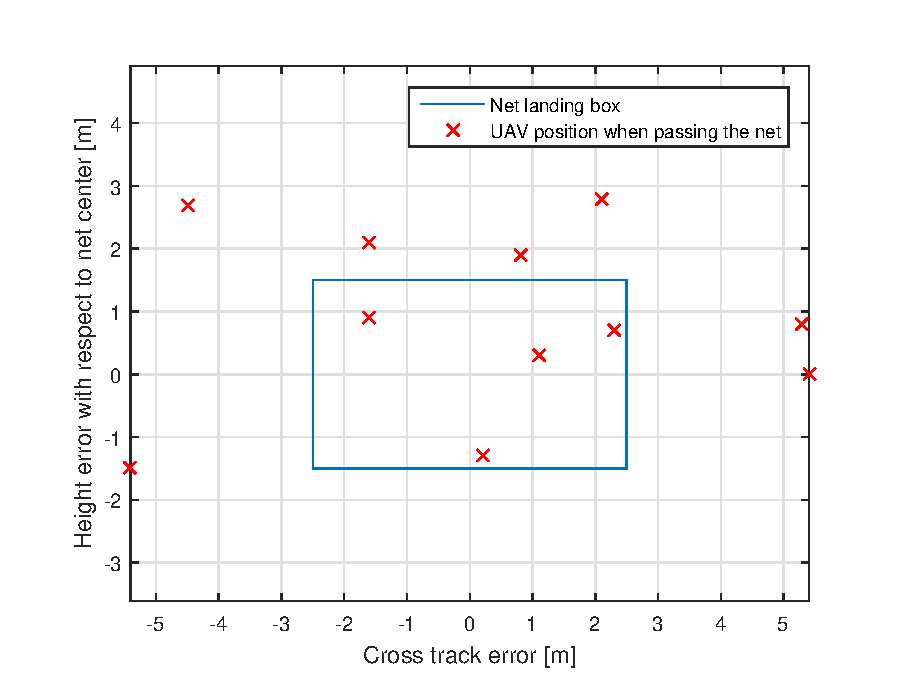
\includegraphics[scale=0.7]{figs/Experiment/day1NetHit.eps}
\caption{Position of UAV relative to the net center at the time of net passing}
\label{Fig:Day1NetPass}
\end{figure}
\subsection{Day 2}
The wind condition on the second day was calm, which allowed for testing the performance of the landing system under ideal conditions.

Observation from the airfield is that the minimum altitude of the \gls{uav} during a landing from east is $56 m$ with the current landing path design. The height controller used saturates in the desired pitch when trying to follow slope at $6 \deg$. A landing path with the maximum slope angle of $6 \deg$ would require a landing path of $700 m$. The the current length of the glide slope the slope angle has to be $11 \deg$. However with a large slope angle the \gls{uav} will quickly gain speed, which will cause a large overshoot at the desired height if not accounted for.

The lateral controller in DUNE performed satisfying during calm wind condition, where the overshoot in the start of each landing plan could have been cause by a bug in the value of the desired height value. However the performance during stronger wind condition cause that the controller to struggle, which is visible during the $180 \deg$ turn. The rapid transition of points during a turn affect the controller with having to recalculate the bank angle during the turn, where a better solution would be to try to keep the bank of the \gls{uav}. This would require the controller to know all the point in the follow path manoeuvre, without breaking the modular boundaries in the DUNE environment.
\subsubsection{Summary day 2}
\begin{table}[H]
\centering
\begin{tabular}{| l | l | l |}
\hline
\textbf{Nr.} 	& \textbf{Mean height error [m]} 	& \textbf{Mean cross track error [m]}  \\ \hline
$1$				& $2.2$							& $3.8$										\\ \hline
$2$				& $1.2$							& $3.4$										\\ \hline
$3$				& $0.9$							& $-1.8$									\\ \hline
$4$				& $2.5$							& $-0.2$									\\ \hline
$5$				& $3.0$							& $0.3$										\\ \hline
$6$				& $1.6$							& $0.2$										\\ \hline
$7$				& $1,9$							& $-2.3$									\\ \hline
$8$				& $1.9$							& $-0.1$									\\ \hline
\end{tabular}
\caption{Mean height and cross track error from day 2}
\end{table}
\begin{figure}[H]
\centering
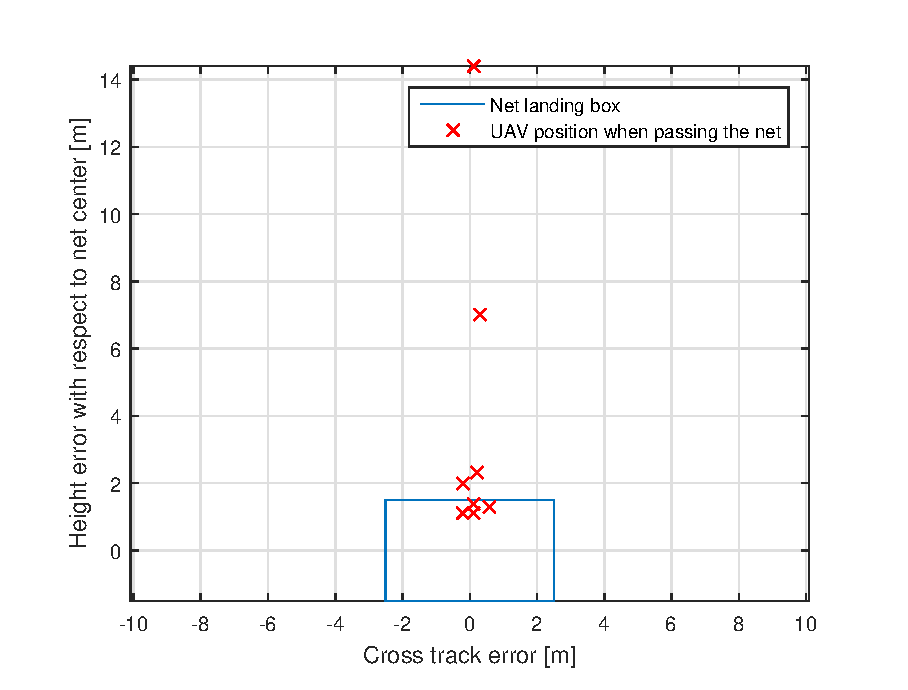
\includegraphics[scale=0.7]{figs/Experiment/day2NetHit.eps}
\caption{Position of the \gls{uav} relative to the net center at the time of net passing}
\label{Fig:Day2NetPass}
\end{figure}
\section{Navigation}\label{ss:EXNavigation}
\subsection{RTK-GNSS performance}
The performance of the \gls{rtk-gnss} system during the first day of executing landing plans is summaries in table \ref{TB:RTKFirstDayLanding}, which shows that \gls{rtk-gnss} kept a stable FIX during the landing plan experiment. The same result was achived during the second day
\begin{table}
\centering
\begin{tabular}{| l | l | l | l |}
\hline
\textbf{Nr.}	& \textbf{FIX \%}	& \textbf{FLOAT \%}	& \textbf{NONE \%}	\\ \hline
$1$				& $99.5 $	& $0.5$	& $0.0$									\\ \hline
$2$				& $99.5 $	& $0.5$	& $0.0$									\\ \hline
$3$				& $99.8 $	& $0.0$	& $0.0$									\\ \hline
$4$				& $100$		& $0.0$	& $0.0$									\\ \hline
$5$				& $100$		& $0.0$	& $0.0$									\\ \hline
$6$				& $100$		& $0.0$	& $0.0$									\\ \hline
$7$				& $99.9$	& $0.1$	& $0.0$									\\ \hline
$8$				& $99.7 $ 	& $0.3$	& $0.0$									\\ \hline
$9$				& $99.3$	& $0.7$	& $0.0$									\\ \hline
$10$			& $100$		& $0.0$	& $0.0$									\\ \hline
$11$			& $100$		& $0.0$	& $0.0$									\\ \hline
\end{tabular}
\caption{Performance of the RKT-GNSS system the first day during the executing of the landing plans}
\label{TB:RTKFirstDayLanding}
\end{table}
\subsection{Short loss compensator}
\begin{figure}
\centering
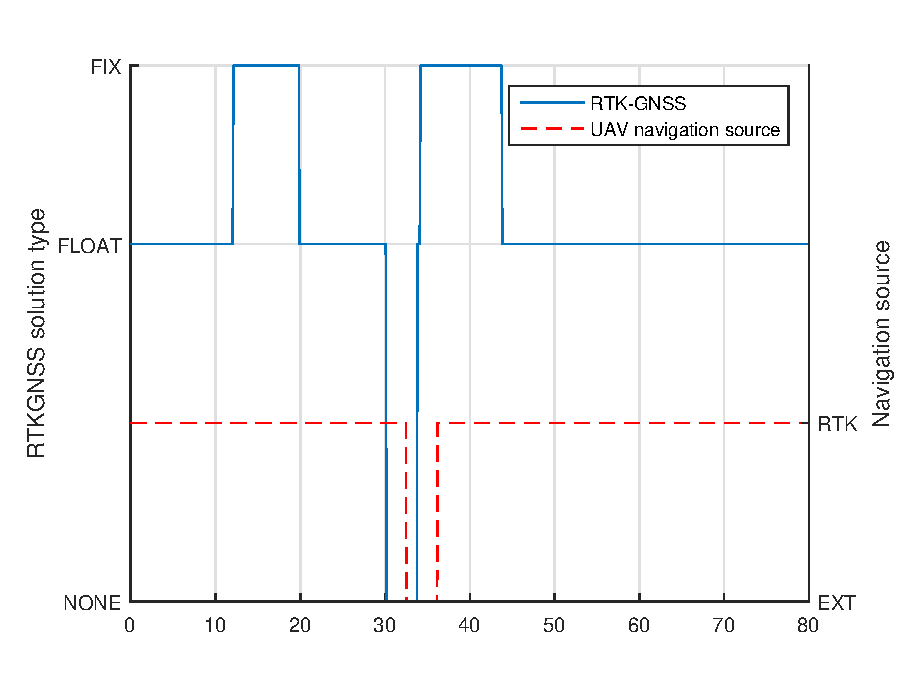
\includegraphics[scale=0.7]{figs/Experiment/navSource.eps}
\caption{State of RTK-GNSS system and \gls{uav} navigation source}
\label{Fig:NavSource}
\end{figure}
\begin{figure}[H]
\centering
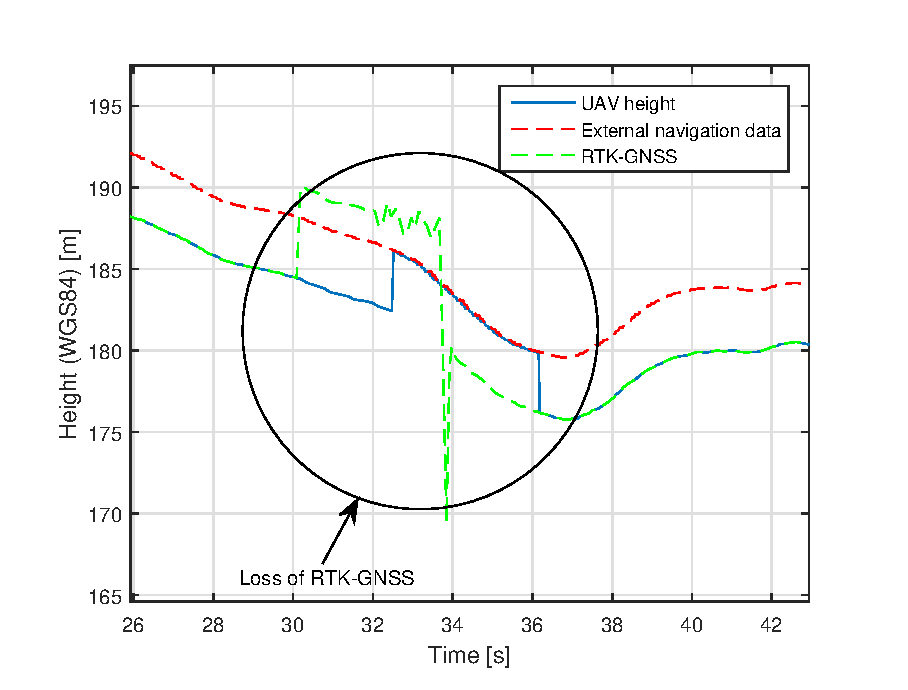
\includegraphics[scale=0.7]{figs/Experiment/shortrtkloss1juni114124.eps}
\caption{Loss of \gls{rtk-gps} triggers the short loss compensator such that the \gls{uav} keeps the \gls{rtk-gps} position solution longer}
\label{Fig:ShortLoss}
\end{figure}
\section{Summary} 